\documentclass[preprint,12pt,authoryear]{elsarticle}
%\documentclass[final,1p,times,twocolumn,authoryear]{elsarticle}
\usepackage{lineno,hyperref}
\modulolinenumbers[5]

\journal{Journal of \LaTeX\ Templates}

%%%%%%%%%%%%%%%%%%%%%%%
%% Elsevier bibliography styles
%%%%%%%%%%%%%%%%%%%%%%%
%% To change the style, put a % in front of the second line of the current style and
%% remove the % from the second line of the style you would like to use.
%%%%%%%%%%%%%%%%%%%%%%%

%% Numbered
%\bibliographystyle{model1-num-names}

%% Numbered without titles
%\bibliographystyle{model1a-num-names}

%% Harvard
\bibliographystyle{model2-names.bst}\biboptions{authoryear}

%% Vancouver numbered
%\usepackage{numcompress}\bibliographystyle{model3-num-names}

%% Vancouver name/year
%\usepackage{numcompress}\bibliographystyle{model4-names}\biboptions{authoryear}

%% APA style
%\bibliographystyle{model5-names}\biboptions{authoryear}

%% AMA style
%\usepackage{numcompress}\bibliographystyle{model6-num-names}

%% `Elsevier LaTeX' style
%\bibliographystyle{elsarticle-harv}
%%%%%%%%%%%%%%%%%%%%%%%

\begin{document}

\begin{frontmatter}

\title{algorithms vs. surveyors: a comparison of automated landform delineations and surveyed landform position in an Alpine environment}


%% Group authors per affiliation:
\author{Fabian E. Gruber\fnref{myfootnote}}
\author{Jasmin Baruck\fnref{myfootnote}}
\author{Clemens Geitner\fnref{myfootnote}}

\address{University of Innsbruck}

\begin{abstract}
Landform delineation has long been used in digital soil mapping to infer soil-relevant information. While its potential as an environmental variable in soil parameter modeling has been investigated for various automated landform delineations, little research has been invested into the relationship between the delineation of landforms by algorithms based on digital terrain models and the perception of landforms by the soil surveyor during field work. Five automated landform classification algorithms and a support vector machine classifier based on single terrain parameters are investigated  with regard to their ability to replicate topographic position, at two different scales, as described by surveyors for soil profile sites in South Tyrol. While a clear trend regarding grid cell size and window size can be observed with regard to the difference between macro and meso scale topographic positions, the overall classification accuracy regarding the different topographic position classes was less promising. Although some automated classifications partly resemble the surveyor's classification, a considerable number of issues remain to be investigated in order to explain the lack of reproducibility of surveyor position, some of which are linked to Alpine environment of the study area.  These include the dominance of the backslope position, the objectivity of the surveyor in rugged terrain under forest, and the fuzzy nature of classifying topographic position. By applying a forward stepwise feature selection procedure, we show that at macro scale a regional terrain parameter (topographic wetness index) and curvatures at a coarse DTM resolution are the most influential in distinguishing topographic position, whereas at meso scale it is the topographic position index with a search radius of just 70 m together with slope.  
 
\end{abstract}

\begin{keyword}
landform delineation, topographic position, automated landform classification, soil profile site description.
\end{keyword}

\end{frontmatter}

\linenumbers

\section{Introduction}
Topography has always been acknowledged as an important control on the formation and, hence, distribution of soil. \cite{Schaetzl2013} notes that by solely discussing a soil based on the description of a pit face, a soil surveyor disregards the possibly most influential factor in its formation - the landscape.	Consequently, soil description guidelines for soil classification schemes require the characterization of landform and topography of soil profile sites. For instance, when following the FAO guildines for soil description, topography is described using the four categories major landform, relative position of the site within the landscape, slope form and slope angle \citep{FAO2006}. Similarily, the Austrian \citep{Nestroy2011} as well as the German soil classification and mapping manuals \citep{ArbeitsgruppeBoden2006} require the measurement of slope angle and a description of the landform on which the soil profile site is located at three different (macro, meso and micro, relative to the surrounding 100 to 500 m, 50 to 100 m and 5 to 10 m, respectively) scales \citep{Englisch1998}. The various landform and slope position descriptions are usually performed by the surveyor while at location, supported by topographic maps and possibly aerial photographs, and based on expert rule sets as well as the surveyor's mental soil landscape model. 

Readily available digital terrain models (DTMs) of increasing resolution have led to reasearch into landform modeling and the segmentation or stratification  of DTMs into landform units. Approaches vary from expert-based rulesets to completely automated landform classifications, from supervised to unsupervised classifications, and include classifications with crisp as well as fuzzy borders.  The output units may be attributed with the names of landforms as mapped by a surveyor, but can also represent elementary land units that adhere to certain geometric constraints. Similar to the information required of the soil surveyor (slope angle and landform), the input variables for DTM-based landform classifications range from local terrain variables, such as slope and curvature, to regional variables like catchment area, which further describe a profile site's position in the landscape.

An early example of the local terrain variable approach was  proposed by \cite{Dikau1988}, who  combined plan and profile curvature as well as the radius of curvature to create a map of form elements. \cite{Pennock1987} describe a similar landform element classification based on plan and profile curvatures. Adressing the problem of appropriate scale, \cite{Wood1996} presented an approach based on slope and multiple curvature calculations to model 6 morphometric features, and added the possibility to calculate the terrain parameters at different scales, i.e. at different window sizes. A similar analysis with regard to curvature and slope was performed by \cite{Blaszczynski1997}.  \cite{Minar2008} proposed a concept of elementary landforms on the basis of homogeneous areas  of  altitude and its derivatives, separated by lines of discontinuity.  

Another branch of landform classifications applies not only local, but also regional terrain attributes \citep{Gallant2000} that include information on the surrounding area of a central pixel. \cite{Schmidt2004} extendet Dikau's form elements by means of fuzzy classification and  introduced landscape context into the classification scheme by implementation of the TOP HAT approach \citep{Rodriguez2002} to additionally distinguish between valleys and hills.  Similarily, \cite{MacMillan2000a} proposed a landform element classification based on heuristic rules and fuzzy logic. Therein, the landform elements of \cite{Pennock1987} are classified based on a semantic input model, and landscape context is added via terrain parameters that describe each cells slope position relative to its watershed. \cite{Klingseisen2008} present a landform classification based on classic local terrain attributes as well as elevation-related regional attributes. The slope class is further segmented using breakpoints in the slope profile. In a similar approach, \cite{Matsuura2012} also applied breakpoint detection to create subdivisions of the slope class.  \cite{Hollingsworth2006} is an example for an application of regional terrain parameters in landform classification that can be linked to the hydrological regime, as they use the Static Wetness Index in their decision tree based, land unit mapping approach. \cite{Weiss2000} proposed an automated landform classification by combining the Topographic Position Index (TPI), which compares the elevation of a pixel to that of surrounding pixels, at large and small scale. Involving the surrounding landscape at a given search radius, r.geomorphons \citep{Jasiewicz2013} represents a classification based on line-of-sight calculations and pattern recognition.

The previously mentioned landform classification approaches have in common that the resulting classes  are attributed names which have specific implications regarding the description or characterisation of each landform element. A different approach is unsupervised classification, wherein an algorithm seperates the grid cells into classes that may or may not be afterwards provided with a name attribute related to landforms. Instead of organising a map according to certain heuristic rules, unsupervised classifications create groups of grid cells that are similar with regard to certain terrain parameters, but the group boundaries are not constrained by any existing classification system. \cite{Irvin1997} compared the results of a crisp and a continuous clustering algorithm with regard to manually delineated landforms.  While \cite{Adediran2004}, \cite{Arrell2007} and \cite{Burrough2000a}  similarily applied clustering of terrain derivatives with regard to landforms, \cite{Moravej2012} based their clusters not on the terrain attributes but on their first principle components. A different unsupervised approach is that of  \cite{Iwahashi2007}, who applied a nested-means partitioning algorithm to delineate terrain types or surface-form classes.

Yet another approach to landform delineation is derived from object-based image analysis (OBIA), its principles applied to geographic information science are described by \cite{Blaschke2014}. It differs to the previously described approaches, as in a first step homogenous areas with regard to certain terrain parameters are segmented, which can later be aggregated and classified into landfrorm elements. \cite{Dragut2006} classified landform elements similar to the concepts of \cite{Dikau1988} and \cite{Pennock1987} by applying OBIA  to a group of terrain parameters which has been used in many landform classification attempts, i.e. slope, plan and profile curvature, and  elevation. \cite{Gercek2011}, \cite{Mashimbye2014} and \cite{Kringer2009}  provide further examples of the application of OBIA to landform delineation, the latter for use in soil mapping procedures.

Geomorphology may be the main subject of interest for automated landform classification, nonetheless the relationship between landforms and soil has long been of strong scientific interest, consequently leading to research into classifying landforms for soil mapping purposes \citep{Schmidt2004,Herbst2012,Hughes2009, Barringer2008}. \cite{MacMillan2000a} well illustrate how different landforms can be interpreted in terms of soil formation and erosion, and the concept of the catena in soil science \citep{Schaetzl2013} shows the importance of topographic position in pedogenesis. Many have highlighted the importance of topography as a soil forming factor especially in Alpine areas \citep{Geitner2011,Herbst2012}. Consequently, it seems important, especially for future research, to consolidate the perception of topographic position in field soil survey on the one side and digital terrain analysis on the other, in order to advance the understanding of the interdependencies between soil and topography.

The aim of this study is to test various landform classification algorithms with regard to their suitability to emulate the mental soil-landscape model of soil surveyors, especially with regard to the concept of topographic position. The resulting map of topographic position may serve as an additional support for soil surveyors during field work. Whereas past publications presenting new landform classification approaches commonly measure the performance of their classification by visual or statistical comparison with existing thematic maps (or classifications performed by human interpretation of photo- or topographic maps for validation purposes) or by correlation with metric parameters such as soil depth, the authors deemed in it important to analyse the classifications performed during field work. Consequently, in this study we compare computed classifications to the topographic positions of numerous soil profile sites in South Tyrol (Italy) as mapped by soil surveyors. The Alpine environment of this research area presents an additional challenge to automated landform classification, as most previous studies have concentrated on areas suited for agriculture, thus having significantly less distinguished elevation differences as well as slope gradients.

The investigated algorithms were restricted to supervised classifications implemented in the readily available Open Source geographic information systems (GIS) GRASS GIS \citep{GRASS_GIS_software} and SAGA GIS\citep{conrad2015system}.  Although some classifications have been compared with the results of different algorithms, and \cite{Barka2011} compared a number of automated landform classification algorithms with regard to correlation with soil and forest units, to our knowledge there has been no systematic comparison to point classifications by surveyors. Furthermore, in this study we investigate the topographic position not only at one, often not clearly defined, scale, but specifically at meso as well as macro scale as defined in the survey manual used by the surveyors \citep{Englisch1998}.

 For each algorithm, a stepwise forward feature selection using support vector machines (SVM) is applied to derive the parameter combination of each classification algorithm best suited to classify the landscape according to the surveyors mental model. Additionally, we examine how changes to the individual model parameters affect the distribution of landform classes and how they are attributed to the various topographic positions. Applying a feature selection procedure further allows to investigate whether a multi-scale approach is beneficial for any of the different landform classifications. By applying this procedure to single terrain derivatives, we investigate how combinations of these derivatives compare to automated classifications and highlight those terrain parameters and landform classifications that contribute most to the description and separation of landforms and slope positions.
\section{Material and Methods}
\subsection{Forestry Service point data set}
The point data set used in this study was provided by the Department of Forestry Planning of the Autonomous Province Bolzano, South Tyrol (Italy).
The data set includes 1968 points with known coordinates (Figure \ref{fig:datapoints}), spread over all of South Tyrol, ranging from the colline to the alpine elevation zone. Nevertheless, the flat valley bottoms are under-represented in the data set, as they are used for agriculture and orchards rather than forestry, which is restricted to slopes and higher altitudes.
\begin{figure}
\includegraphics[width=\textwidth]{suedtirol.eps}
\caption{Map of South Tyrol showing the locations of the soil profile sites of the Forestry Service data set. }
\label{fig:datapoints}
\end{figure}
 This point data set is the result of  various projects of the Forestry Departement, the most substantial part coming from the Forestry Survey \citep{APB2006}. Additionally to the silvicultural description of each site, the data set contains a soil profile description for most of the points. Part of the soil profile site information is a description of the topographic position. Figure \ref{fig:hist} shows the distribution of the profile sites' topographic positions at different levels of generalisation for macro and meso scale.

\begin{figure}
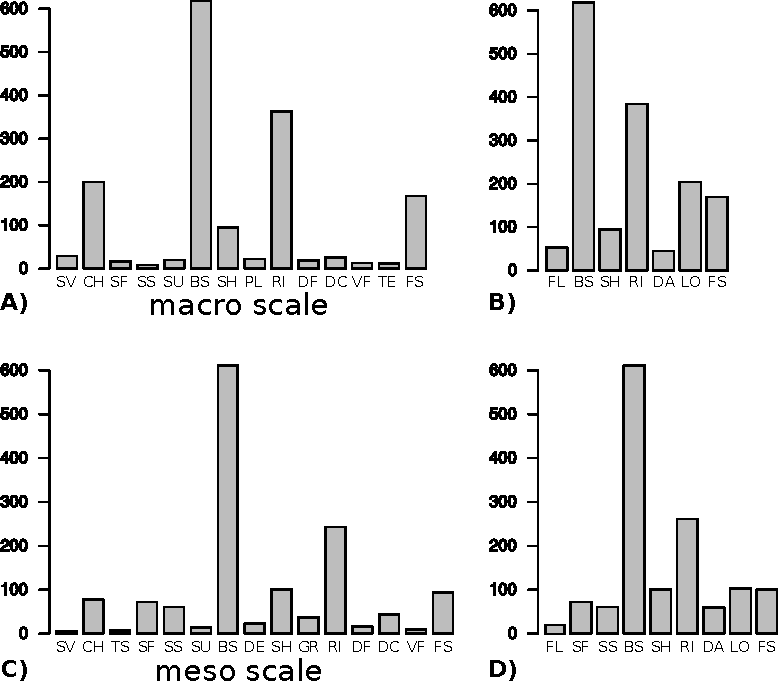
\includegraphics[width=\textwidth]{Distribution_of_topographic_position_EDITED_onlyGL1.pdf}
\caption{Distribution of the topographic positions of the profile site data points at macro (A,B) and meso (C,D) scale. The histograms on the left show the detailed topographic positions from the survey, while B and D show the generalisations applied at macro and meso scale, respectively. See Tables \ref{table:topopositions} and \ref{table:generalisations} for the abbreviations of topographic position. }
\label{fig:hist}
\end{figure}

1668 profile descriptions include  the topographic position at macro scale, 1468 at meso scale and only 108 additionally provide information on micro-scale topographic variability. The survey was performed adhering to the Forestry Survey Manual \citep{Englisch1998}, where the classes for the topographic position at macro and meso scale are mostly the same, with the difference that the former is attributed to the area within 100 to 500 m of the soil profile site, while the latter is judged based on the topography of the area within 50 to 100 m. For this study, the topographic position classes were generalised into fewer classes to simplify  analysis and classes with very small numbers of members were removed. Table \ref{table:topopositions} gives an overview of the original classes of the Forestry Survey and describes the generalisation applied for this study. The classes slope flattening and slope steepening were only analysed at meso scale.
\begin{table}[!htbp]
\caption{Overview of the topographic positions and their description for the surveyor (according to \cite{Englisch1998}) as well as the generalised classification applied in the study. "-" signifies that the class members were removed from the analysis.}
\begin{center}    \begin{tabular}{  p{3cm} c p{7cm} c }
	\hline
	Topographic position & Abbrev. & description for surveyor & gen. class \\ \hline
	plane &EF& expanded flat area  & FL \\ \hline
	locally flat &LF&	small flat area  & FL \\  \hline
	valley floor &VF& flat area bounded by upward slopes  & FL \\  \hline
	\raisebox{-0ex} {terrace} &\raisebox{-0ex}{TE} & flat area bounded by one upward and one downward slope  & FL \\   \hline
	plateau &PL& flat area bounded by downward slopes  & FL \\   \hline
	depression &DE& circular concave landform & LO \\   \hline
	pan &PA& oval concave landform & LO  \\   \hline
	channel &CH& Elongated concave landform  & LO\\   \hline
	shoulder &SH& convex landform with erosion dominating & SH \\   \hline
	footslope &FS& concave landform with accumulation dominating  & FS\\   \hline
	backslope &BS& erosion equals accumulation & BS  \\   \hline
	slope steepening &SS& slope bounded by areas with lesser slope gradient  & SS \\   \hline
	slope flattening &SF& slope bounded by areas with larger slope gradient & SF \\   \hline
 	summit &SU& circular convex landform & RI \\   \hline
	ridge &RI& oval convex landform  & RI\\   \hline
	rampart &RA& elongated convex landform  & RI\\   \hline
	toeslope &TS& concave transition from footslope to flat & FS \\   \hline
	debris fan &DF& gently sloping mound from gulley accumulation & DA  \\   \hline
	debris cone &DC& Steep sloping mound from gulley accumulation  & DA\\   \hline
	interchanging gulleys and ridges &\raisebox{-1.5ex} {GR} & \raisebox {-1.5ex} {interchanging gulleys and ridges} & -  \\  \hline
	secondary valley flanks &\raisebox{-1.5ex}{SV}& \raisebox{-1.5ex}{secondary valley flanks}  & - \\   \hline
    \end{tabular}
\end{center}	
\label{table:topopositions}
\end{table}

\subsection{Automated landform classification algorithms}
The base input for the landform classification is a digital terrain model (DTM) with a grid size of 2.5 m, the result of an airborne laser scanning mission \citep{Wack2005}. It is freely available for download at the homepage of the \cite{DTM}. For use in this study the DTM was resampled to 10, 50, 100 and 150 m to consider the influence of scale. The methodology was not applied to the original DTM due to computational limits regarding such a regional approach. The following automated landform classification algorithms were performed on these DTMs applying a wide range of parameter settings:
\paragraph{Dikau's curvature classification \citep{Dikau1988}}
Dikau's proposition of a geomorphographic system of classifying landforms includes a classification of landform elements based on horizontal and vertical curvature. Depending on whether a grid cell is classified as convex, concave, or  planar with regard to these two directions, it is given membership to one of nine classes of landform element types. This classification is implemented in the SAGA Tool ``Curvature Classification''. The threshold value for distinguishing between planar and convex or concave is the only parameter open to variation. \cite{Hoersch2002} used this approach to correlate topography with the spatial distribution of vegetation. \cite{Jasiewicz2013} evaluated and compared their landform classification algorithm ``r.geomorphon'' with Dikau's curvature classification.
\paragraph{Wood's morphometric features \citep{Wood1996}}
The calculation of this classification was performed using the algorithm implemented in the GRASS GIS 7  add-on ``r.param.scale''.  For a chosen window size it computes a number of terrain parameters by fitting bivariate quadratic polynomials.  The classification of each grid cell into the classes planar, pit, channel, pass, ridge and peak is performed based on the parameters slope and curvature, specifically cross-sectional, longitudinal, maximum and minumum curvature. A variation of  the slope and curvature thresholds is possible for the classification into the six morphometric features.
\cite{Bolongaro-Crevenna2005} applied Wood's morphometric features and compared the distribution of the morphometric features for traditionally mapped landforms in Morelos State, Mexico, using double ternary diagrams. \cite{Ehsani2008} compared the results of Wood's classification algorithm with landform elements extracted using  an unsupervised Artificial Neural Networks agorithms based on the the same slope and curvature parameter maps. Both aforementioned studies discuss the choice of approriate thresholds for slope and curvature. \cite{Ehsani2009} extended their previous study  to include Landsat ETM+ bands in their analysis.  
\paragraph{Fuzzy landform elements \citep{Schmidt2004}}
While Dikau's curvature classification is based on local terrain parameters, \cite{Schmidt2004} extended this approach be evaluating the resulting form elements with regard to their landscape context.  Instead of horizontal curvature, tangential curvature is used for the classification of form elements in slopeing areas, analogous to Dikau's procedure, and maximum and minimum curvature are included for the classification of flat areas analogous to Wood's parametrization \citep{Wood1996}. Fuzzy classification is applied for differentiating sloping and flat areas as well as the different form elements. The fuzzy classification of these landform elements is implemented in the SAGA GIS tool “Fuzzy landform classification”. The parameters varied in the present study are the fuzzy classifiers for slope and curvatures. \cite{Schmidt2004} further present an extension of this approach involving landscape context by including a TOP HAT ridge and valley detection \citep{Rodriguez2002}  to differentiate the hillslope position of the landform elements into hill, hillslope and valley. These landform elements have been used in modeling rooting depth \citep{Schmidt2004} and in  soil-landscape modeling \citep{Schmidt2005}. \cite{Hughes2009} applied  the landform elements for modeling the distribution of loess in North Otago, New Zealand, with promising results regarding primary loess. Mokkaram et al. (2005) compare this fuzzy classification of slope and curvatures to TPI-based landforms, with regard to their relationship to the units of a geological map.
\paragraph{Topographic position index (TPI) and TPI-based landform classification \citep{Weiss2000}}
The TPI is defined as the difference between the elevation of a central grid cell and the mean elevation of the surrounding grid cells with any given search radius and thus defines the relative position of the grid cell along a topographic gradient \citep{Guisan1999}. \cite{Weiss2000} developed a system that classifies a grid cell into one of ten landform classes based on the combination of a large scale TPI and a small scale TPI, i.e. one with a large and one with a small search radius.  On its own, the TPI has been applied in different fields, for instance \cite{Gercek2010} used the TPI in an object-based approach to delineate landform elements for mapping land management, while \cite{Reu2013} analyse its application in an geoarcheological setting. While \cite{Mokarram2015} compared TPI-based landforms to Schmidt's fuzzy landforms, \cite{Barka2011} analysed the TPI-based landform classification as well as other landform classifications with regards to  soil and forest units.
\paragraph{Geomorphon-based landform classification \cite{Jasiewicz2013}}
This pattern recognition – based landform classification is implemented through the GRASS GIS 7 add-on “r.geomorphon”. It performs line-of-sight calculations in the direction of the 8 neighboring grid cells.  Depending on whether the line-of-sight ends downwards,  upwards, or in the flat, this direction is attributed “-”,”+” or “0”, respectively.  Based on this ternary pattern, each grid cell can be classified as one of ten landform elements. The two parameters considered in this research are the search distance (L), up to which the line-of-sight computations are performed as well as the slope angle (flat) that constitutes the threshold up to which a direction is classified as flat. 

\subsection{Statistical methods}
The extraction of the parameters for each classification that result in a landform classifications that best corresponds to that of the surveyor, was performed by applying support vector machine classification in a forward stepwise feature selection procedure.
\paragraph{Support vector machine classification}
SVM classification was introduced by \cite{Cortes1995} as a binary classifier. The basic idea is to find a hyperplane that best seperates the points of two classes by maximizing the margin between those points of both classes that are closest to each other, called support vectors. A tuning parameter $C$ allows for certain violations of this margin, thus increasing the number of support vectors by those points that are on the "wrong" side of this (soft) margin. This simple approach for linear boundaries is extended to the nonlinear case using kernels to increase the feature space. For this study, SVM classification was performed using the "e1071" package \citep{meyer2014} of the statistical computing environment R \citep{cran2014} with a radial kernel and 10-fold cross-validation. Variation of the tuning parameters gave  no reason to defer from the default parameter setting. Multiclass-classification applies a one-against-one approach, thus fitting each class against each other and then attributing the appropriate class to each point. Examples for consideration and application of SVMs with regard to soil mapping are \cite{Ballabio2009}, \cite{Behrens2006} and \cite{Rossel2010}.
\paragraph{Parameter selection procedure} For each group of automated landform classifications as well as one group of single local and regional terrain parameters, the best fitting parameter combination was investigated by applying a stepwise forward selection approach. In a first step, the parameter combination that on its own best fits the surveyor's classification was chosen based on minimum classification error. In the next step each of the remaining parameter combinations were added to the model to find the combination that best improved the original (single parameter combination) model. Ten-fold cross validation was performed for each step as well as for the entire parameter selection procedure. The meaningfulness of this feature addition was evaluated using the "one-standard-error-rule" \citep{James2013} as well as visual inspection of the scree plots, as exemplified in the workflow diagram in Figure XXX, in order to choose a minimum of parameters to simplify interpretation. Overall prediction error was chosen as accuracy measure for the parameter selection process because the application of Cohen's kappa index requires simple random sampling \citep{Congalton1991}, whereas the profile sites in the data set of this study weres sampled mostly for practical reasons. Furthermore, \cite{Pontius2011} argue that kappa seldom adds additional information to overall accuracy.ISTHATTOOHARSH?
\section{Results}
\subsection{Dikau's curvature classification}
Dikau's landform element classification scheme produces a map containing the classes V/V, GE/V, X/V, V/GR, GE/GR, X/GR, V/X, GE/X, X/X, where the first letter describes the profile curvature as being convex (X), concave (V) or elongated (GE), while the second letter of the class name describes the planar curvature as planar (GR), X or V.

\begin{table}[!htbp]
\caption{Accuracy values of  Dikau's curvature classification maps computed  with the best parameter setting for each topographic position. res = DTM resolution, tc = curvature threshold for plane, Ov = Overall accuracy}
\centering
\begin{tabular}{p{2.1cm}|cccccccccc}
  \hline
  \hline
macro scale & FL & LO & DA & FS & SF &  BS & SS & SH & RI & Ov \\ 
  \hline
res=100m tc=0.006  & \raisebox{-0ex}{0.00} & \raisebox{-0ex}{0.49} & \raisebox{-0ex}{0.20} & \raisebox{-0ex}{0.00} &-& \raisebox{-0ex}{0.81} &-& \raisebox{-0ex}{0.00} & \raisebox{-0ex}{0.37} & \raisebox{-0ex}{0.49}\\ 
 \hline
 \hline
meso scale & FL & LO & DA & FS & SF & BS & SS & SH & RI & Ov \\ 
  \hline
{res=50m tc=0.007} & {0.00} & {0.26} &{0.00} & {0.00} & {0.00} & {0.93} & {0.00} & {0.0} & {0.21} & {0.47} \\ 
 \hline
\end{tabular}
\label{table:dikau}
\end{table}
 At macro scale, the single curvature classification map that best represents the surveyors topographic position at both levels of generalisation is based on the 100 m DTM and applies a curvature threshold for plane of 0.006. This map results in a cross validated overall accuracy of 45\% with the landform elements GE/GR being mapped to the topographic position BS, while the classes GE/V and VV are attributed to the position LO, V/GR to FS and the classes GE/X, X/GR and X/X to the topographic position RI. The position FL, DA and SH are not mapped in this parameter setting and most of the members of the classes LO, FS, SH and RI are misclassified as BS, which dominates the resulting landform classification. At a DTM resolution of 10m the position BS is distributed over all of the classes of the curvature classification, leading to all of these classes being attributed to the class BS. With increasing grid cell size the dominance of the curvature class GE/GR increases and the overall number of mapped curvature classes decreases, resulting in the misclassification of most topographic positions as BS. An increase of plane threshold leads to a reduction of mapped curvature classes, resulting in a decline in correctly classified RI positions, while a decreasing threshold leads to a more balanced distribution of curvature classes, increasing the misclassification of the less dominant topographic position classes to BS. The addition of a further predictor mapset with a different parameter setting leads to no substantial increase in the correct classification rate of surveyed topographic position.
At meso scale topographic position, a similar plane threshold (0.007) returned the best results, however at a finer DTM resolution of 50 m. The curvature classes GE/GR, GE/V, GE/X, V/GR, V/X, X/GR and X/V are all mapped to the topographic position BS. Only the more extreme curvature combinations V/V and X/X are mapped to different topographic positions, LO and RI respectively. As is the case at macro scale, an increase in DTM resolution leads to a more diverse distribution of the points with a backslope position amongst the curvature classes, and consequently decreases the landform classification's ability to distinguisch the backslope position from the other topographic positions. Table \ref{table:dikau} gives an overview of the best parameter settings for both scales.

\subsection{Wood's morphometric features}
Wood's landform classification algorithm yields a map containing the six morphometric features planar, pit, channel, pass, ridge and peak. Table¸\ref{table:wood} gives an overview of the best parameter settings for woods morphometric features.
At macro scale, the parameter setting that returns the classification which best corresponds to the surveyed classes is based on the 50 m DTM, a window size of 250 m, a curvature threshold of 0.002 and a slope threshold of 14 degrees. This however results in a map containing only the morphometric features channel, planar and ridge, which are consequently mapped to the surveyed topographic positions LO, BS, and RI, while all other positions are not recreated. An increase in window size only leads to further misclassification to the position BS, decreasing the number of points mapped to the position LO and eliminating all RI positions. A reduction of window size or, similarily, an increase in DTM resolution leads to an increase in the number of morphometric features. As a consequence, points with the topographic position BS are more evenly distributed on the different morphometric features, diminishing the maps ability to distinguish between BS and the other topographic positions, resulting in misclassification to the BS class. A reduction of the planar curvature threshold leads to similar results, while an increase leads to patterns similar to those associated with an increase in window size. While raising the slope threshold increases the number of points classified as BS at the cost of the remaining two classes LO and RI, a reduction leads to slightly less points classified as LO and a small increase of the proportion of the morphometric feature ridge. 
\begin{table}[!htbp]
\caption{Accuracy values of  Wood's parametric feature maps computed  with the best parameter setting, for each topographic position at macro  and meso scale. "plus"  indicates that the parameter setting described is combined with the aforementioned parameter setting. res = grid cell size, ws = window size, ts = slope threshold, tc = curvature threshold, Ov = Overall accuracy}
\centering
\begin{tabular}{p{2.8cm}|cccccccccc}
  \hline
  \hline
macro scale & FL & LO & DA & FS & SF &  BS & SS & SH & RI & Ov \\ 
  \hline
res=50m ws=250m ts=14 tc=0.002 & \raisebox{-1.5ex}{0.00} & \raisebox{-1.5ex}{0.39} & \raisebox{-1.5ex}{0.00} & \raisebox{-1.5ex}{0.00} &\raisebox{-1.5ex}{-} & \raisebox{-1.5ex}{0.80}&\raisebox{-1.5ex}{-} & \raisebox{-1.5ex}{0.00} & \raisebox{-1.5ex}{0.36} & \raisebox{-1.5ex}{0.46}  \\ 
 \hline
 \hline
meso scale & FL & LO & DA & FS & SF & BS & SS & SH & RI & Ov \\ 
  \hline
res=10m ws=110m ts=11 tc=0.006 & \raisebox{-1.5ex}{0.00} & \raisebox{-1.5ex}{0.39} & \raisebox{-1.5ex}{0.00} & \raisebox{-1.5ex}{0.00} & \raisebox{-1.5ex}{0.00} & \raisebox{-1.5ex}{0.90} & \raisebox{-1.5ex}{0.00} & \raisebox{-1.5ex}{0.00} & \raisebox{-1.5ex}{0.25} & \raisebox{-1.5ex}{0.47} \\ 
 \hline
\end{tabular}
\label{table:wood}
\end{table}

At meso scale, two parameter settings tied with regard to best overall cross-validated accuracy at 47\%. While both only predict the topographic positions LO, BS and RI, the setting with  larger window size (150 m compared to 110 m), higher slope threshold (13 compared to 11) and lower curvature threshold (0.004 compared to 0.006)performed slightly better for the position RI, whereas the other setting performed slightly better for LO and BS. The effects of changes to the parameters window size as well as slope and curvature threshold are comparable to those at macro scale. Additional parameters sets yield no significant improvement.

\subsection{Fuzzy landform elements}
Schmidt's fuzzy landform classification expands Dikau's curvature classification by introducing the terrain parameters minimum and maximum curvature and fuzzy membership functions. This results in a map where each grid cell is attributed one of the classes termed "foot hollow", "hollow", "shoulder hollow", "footslope", "back slope", "shoulder slope", "foot spur", "spur", "shoulder spur", "plain", "channel", "pit", "ridge", "saddle" and "peak".
Regarding the topographic position at macro scale, the parameter setting that produced the map that best corresponds to the surveyed position relied on the 150 m DTM and lower and upper slope thresholds for the semantic input models of 6 and 12 degrees, respectively (Table \ref{table:fuzzy}). The thresholds for curvature that establish fuzzy membership to the classes straight and curved were chosen to be 0.0001 and 0.003. This parameter setting failed to reproduce correctly any of the data points of the classes DA and SH and achieved an overall accuracy of 48\%. The resulting map attributes the fuzzy class "plain" to the topographic position FL and the classes "foot hollow" and "hollow" to LO. The classes "foot slope" and "back slope" are mapped to the positions FS and BS, respectively, while the classes "spur", "shoulder spur","shoulder slope", "peak" and "pit" are assigned the topographic position RI. Reducing the DTM grid size to 50 m while maintaining the rest of the chosen parameters, increases the number of fuzzy classes eventually mapped to BS from one to nine, which decreases the topographic positions depicted in the resulting map to the positions FL, BS and RI. An increased grid cell size of 250 m further exagerates the membership of data points to the class BS. Changes of plus or minus 3 degrees to the slope thresholds lead to only slightly different results. A reduction of the lower curvature thresholds results in a slight shift of classification from BS to RI, whereas an increase thereof decreases the attribution of points to the classes RI, LO and FS due to misclassification to BS. Landform maps based on a larger upper curvature threshold hardly contain any landform classes except for BS, and to a much smaller extent FL and RI.

\begin{table}[!htbp]
\caption{Accuracy values of  Schmidt's fuzzy element maps computed  with the best parameter setting for each topographic position at macro scale. res = DTM resolution, ts = fuzzy slope thresholds, tc = fuzzy curvature thresholds, Ov = Overall accuracy}
\centering
\begin{tabular}{p{2.8cm}|cccccccccc}
  \hline
  \hline
macro scale & FL & LO & DA & FS & SF &  BS & SS & SH & RI & Ov \\ 
  \hline
res=150m ts=6;12 tc=0.0001;0.003 & \raisebox{-1.5ex}{0.38} & \raisebox{-1.5ex}{0.36} & \raisebox{-1.5ex}{0.00} & \raisebox{-1.5ex}{0.32} &\raisebox{-1.5ex}{-}& \raisebox{-1.5ex}{0.81} &\raisebox{-1.5ex}{-}& \raisebox{-1.5ex}{0.00} & \raisebox{-1.5ex}{0.29} & \raisebox{-1.5ex}{0.49}  \\ 
 \hline
 \hline
meso scale & FL & LO & DA & FS & SF & BS & SS & SH & RI & Ov \\ 
  \hline
res=50m ts=3;21 tc=0.004;0.006 & \raisebox{-1.5ex}{0.00} & \raisebox{-1.5ex}{0.48} & \raisebox{-1.5ex}{0.00} & \raisebox{-1.5ex}{0.12} & \raisebox{-1.5ex}{0.00} & \raisebox{-1.5ex}{0.90} & \raisebox{-1.5ex}{0.00} & \raisebox{-1.5ex}{0.00} & \raisebox{-1.5ex}{0.26} & \raisebox{-1.5ex}{0.49} \\ 
 \hline
\end{tabular}
\label{table:fuzzy}
\end{table}
At meso scale, there is no dominant forerunner amongst the parameter setting, with several maps achieving similar overall accuracies of 48.6\%. The most frequently chosen setting of the cross validation process is based on the 50 m DTM, a slope membership function that is based on the threshold values 3 and 21$^{\circ}$, and relatively large curvature thresholds of 0.004 and 0.006, which are quite consistent in the cross validation process. The mapping of the fuzzy landforms to the topographic positions is comparable to that at macro scale, except that "plain" is mapped to LO instead of FL. Additionally, the topographic position classes SF and SS are not attributed any fuzzy landform classes. A smaller grid cell size of 10 m leads to the BS points being distributed over all fuzzy landform classes, resulting in all of them being mapped to the class BS. The reduction of DTM resolution leads to similar results, however, in this setting the reason is an output map that only contains a small number of different classes, dominantly "back slope" and, to a much smaller degree, "plain". Variation of curvature thresholds leads to comparable changes in landform distribution as at macro scale. Additional parameter settings lead to no improvisation of overall accuracy.
\subsection{TPI and TPI-based landform classification}
The TPI-based landform classification based on the  classification table by \cite{Weiss2000} results in the map units "canyons", "midslope drainages", "upland drainages", "U-shape valleys", "plains", "open slopes", "upper slopes", "local ridges", "midslope ridges", "mountain tops". The cross-validation process at macro scale does not produce a single parameter setting decisivley better than others, but the best settings involved an inner search radius between 60 and 100 m and an outer radius between 250  and 350 m. All settings preferred the 10 m DTM. The single parameter combination that was most frequently at first place applied search radii of 70 and 250 m. This results in a cross-validated accuracy of 47.7\%, where the landform classes "canyons","midslope drainages" and "U-shape valleys" are mapped to the topographic position LO, "plains" is mapped to the position FL and "open slopes" to BS. While the topographic positions DA, FS and SH are not recreated using a single TPI-based landform classification, the surveyed position "RI" is represented by the landform classes "midslope ridges", "mountain tops" as well as "upper slopes". Both an increase and a decrease of the inner search radius lead to increased misclassification of points to "BS". The latter case leads to less mappings of landform classes to the topographic position LO, despite more points of the landform class "U-shape valley", the number of which strongly decreases with increasing inner search radius. Higher values for the outer TPI radius lead to more points being assigned to the landform class U-shape valleys, however, in this setting this landform class is mapped to the topographic position FS instead of LO. The cross-validation process does not imply a significant increase in overall accuracy through addition of a second landform classification based on a different parameter setting.   
\begin{table}[!htbp]
\caption{Accuracy values of  TPI-based landform maps computed  with the best parameter setting for each topographic position. res = DTM resolution, R1 = inner search radius, R2 = outer search radius, Ov = Overall accuracy}
\centering
\begin{tabular}{p{4.5cm}|rrrrrrrrrr}
  \hline
  \hline
macro scale & FL & LO & DA & FS & SF &  BS & SS & SH & RI & Ov \\ 
  \hline
\raisebox{-0ex}{res=10m R1=70m R2=250} & \raisebox{-0ex}{0.26} & \raisebox{-0ex}{0.43} & \raisebox{-0ex}{0.00} & \raisebox{-0ex}{0.00} &\raisebox{-1.5ex}{-}& \raisebox{-0ex}{0.88} &\raisebox{-1.5ex}{-}& \raisebox{-0ex}{0.00} & \raisebox{-0ex}{0.27} & \raisebox{-0ex}{0.48}  \\ 
\hline
\hline
meso scale & FL & LO & DA & FS & SF &  BS & SS & SH & RI & Ov \\ 
   \hline
{res=10m R1=50m R2=90m} & \raisebox{-1.5ex}{0.30} & \raisebox{-1.5ex}{0.32} & \raisebox{-1.5ex}{0.00} & \raisebox{-1.5ex}{0.13} & \raisebox{-1.5ex}{0.00} & \raisebox{-1.5ex}{0.93} & \raisebox{-1.5ex}{0.00} & \raisebox{-1.5ex}{0.00} & \raisebox{-1.5ex}{0.30} & \raisebox{-1.5ex}{0.50} \\ 
 \hline
\end{tabular}
\label{table:tpi}
\end{table}

At meso scale, the feature selection procedure leads to the choice of the TPI-based landform classification map based on the 10 m DTM and inner and outer search radii of 50 and 90 m. In this setting, the members of the topographic position RI belong to the landform classes "midslope ridges", "mountain tops", and "upper slopes". The positions BS, FS, LO and FL are comprised of the landform classes "open slopes", "U-shape valleys", "canyons" and "plains", respectively. This setting leads to a cross-validated accuracy of 49\%, with the topographic posiitons SS, SH, SF,  and DA not being attributed any data points. Increasing the outer radius leads to an increasing number of landform classes, for instance involving data points classified as "local ridges", and a slightly more balanced distribution of the data points amongst the different landform classes. This however leads to more landform classes being incorrectly assigned to the topographic position BS. 

\subsection{Geomorphon-based landform classification}
The automated classification of DTMs with "r.geomorphon" returns a map of maximum 10 landform classes, i.e. flat, peak, ridge, shoulder, spur, slope, hollow, footslope, valley and pit. Similarily to other classification methods, all or only part of the available landform elements are mapped, depending on the research area's topography and the chosen algorithm parameters. 
Regarding macro scale topographic position, the parameter and input combination that on its own best recreates the topographic positions from field survey is based on the 50 m DTM, a search window (L) of 400 m and a flatness threshold of 10 degrees. The resulting landform element map can correctly classify 49\% of the points. A model of topographic position based on this parameter setting maps the landform elements flat to the surveyor's FL, footslope to DA,  hollow and valley to LO, slope to BS, and the elements peak, ridge, shoulder and spur to RI. No points are mapped to FS and SH, as the generated map mostly incorporates the FS points into the BS class, and to a lesser degree, to LO, while SH points are dominantly classified as BS and RI. Beside FS  and SH, RI also shows a strong overlap with BS. Regarding the effects of parameter variation, while a lower flatness threshold increases the amount of points classified as RI rather than BS, an increase in search window has the opposite effect and increases the misclassification of other topographic positions as BS. The addition of the results of a further classification based on a different set of parameters does not significantly improve overall accuracy.

\begin{table}[!htbp]
\caption{Accuracy values of geomorphon-based landform maps computed  with the best parameter setting for each topographic position and scale. res = DTM resolution, L = search radius, fl = flatness threshold, Ov = Overall accuracy}
\centering
\begin{tabular}{p{2.8cm}|rrrrrrrrrr}
  \hline
  \hline
macro scale & FL & LO & DA & FS & SF &  BS & SS & SH & RI & Ov \\ 
  \hline
res=50m fl=10 L=400m & \raisebox{-1.5ex}{0.38} & \raisebox{-1.5ex}{0.49} & \raisebox{-1.5ex}{0.20} & \raisebox{-1.5ex}{0.00} &\raisebox{-1.5ex}{-}& \raisebox{-1.5ex}{0.81} &\raisebox{-1.5ex}{-}& \raisebox{-1.5ex}{0.00} & \raisebox{-1.5ex}{0.37} & \raisebox{-1.5ex}{0.49}  \\ 
 \hline
 \hline
meso scale & FL & LO & DA & FS & SF & BS & SS & SH & RI & Ov \\ 
  \hline
{res=10m fl=8 L=80m} & \raisebox{-1.5ex}{0.00} & \raisebox{-1.5ex}{0.17} & \raisebox{-1.5ex}{0.00} & \raisebox{-1.5ex}{0.00} & \raisebox{-1.5ex}{0.00} & \raisebox{-1.5ex}{0.92} & \raisebox{-1.5ex}{0.00} & \raisebox{-1.5ex}{0.00} & \raisebox{-1.5ex}{0.38} & \raisebox{-1.5ex}{0.49} \\ 
\end{tabular}
\label{table:geom}
\end{table}

At meso scale, the map with the lowest overall classification error rate at generalisation level 1 is based on the 10 m DTM, a search radius of 80 m and a flatness threshold of 8 degrees. Whereas at macro scale the threshold of 10 degrees was dominant amongst the maps with the highest correct classification rate, at meso scale 8$^{\circ}$ are preferred. In this setting the landform elements flat and valley are mapped to the topographic position LO, hollow and slope are mapped to BS, and footslope, ridge, shoulder and spur are mapped to RI. Again the dominant BS falsely incorporates a great amount of other classes, and FL, DA, FS, SF, SS and SH are not attributed any points by the model based on this map. The overall classification rate is comparable to the one at macro scale.  Table \ref{table:geom} shows the accuracies of the best performing maps.


\subsection{Terrain parameters}
The same procedure that was applied for different parameter settings of each classification algorithm was performed for  numerous local and regional terrain parameters, similarily varying parameters such as grid size and search window. At macro scale, the terrain parameter that, on its own, best reproduced the surveyed topographic positions using SVM classification was the topographic wetness index, a regional terrain parameter relating a grid cell's catchment area to its slope. The resulting model correctly classifies 32\% of the topographic positions described as LO, 85\% of BS and 43\% of RI, which leads to an overall cross-validated accuracy of 48\% . The remaining positions FL, DA, FS, and SH are not attributed any data points in the resulting map, their members being misclassified as one the other three positions. Similar to the results of the investigated classification methods, misclassification to the topographic position BS was dominant. The addition of the terrain parameter profile curvature, calculated with the 50 m DTM and a window size of 350 m, improves the cross validated overall accuracy to 49.4\% by correctly classifying 38\% of the data points attributed to the topographic position FS. This parameter combination also introduces the missing topographic positions FL, DA and SH into the resulting maps. The addition of the terrain parameter minimum curvature, based on the 50 m DTM and a window size of 250 m, further strengthens the less common classes FL, LO and DA, increasing the overall cross validated accuracy to 50.6\%.
\begin{table}[!htbp]
\caption{Correct classification rates for maps computed with different predictors sets of terrain parameters for each topographic position at macro scale with a radial kernel. At each generalisation level, the first row shows the results using only the best terrain parameter, whereas the terrain parameters in the rows below are subsequently added to the predictor set, consequently increasing the overall accuracy. res = DTM resolution, ws = window size, Ov = Overall accuracy}
\centering
\begin{tabular}{p{4cm}|rrrrrrrrrr}
  \hline
  \hline
macro scale & FL & LO & DA & FS & SF &  BS & SS & SH & RI & Ov \\ 
  \hline
topographic wetness index res=50m  & \raisebox{-1.5ex}{0.00} & \raisebox{-1.5ex}{0.32} & \raisebox{-1.5ex}{0.00} & \raisebox{-1.5ex}{0.00} &\raisebox{-1.5ex}{-}& \raisebox{-1.5ex}{0.85} &\raisebox{-1.5ex}{-}& \raisebox{-1.5ex}{0.00} & \raisebox{-1.5ex}{0.43} & \raisebox{-1.5ex}{0.48}  \\  
plus profile curvature res=50m ws=350m  & \raisebox{-1.5ex}{0.06} & \raisebox{-1.5ex}{0.26} & \raisebox{-1.5ex}{0.02} & \raisebox{-1.5ex}{0.39} &\raisebox{-1.5ex}{-}& \raisebox{-1.5ex}{0.84} &\raisebox{-1.5ex}{-}& \raisebox{-1.5ex}{0.12} & \raisebox{-1.5ex}{0.40} & \raisebox{-1.5ex}{0.51}  \\ 
plus minimum curvature res=50m ws=250m  & \raisebox{-1.5ex}{0.21} & \raisebox{-1.5ex}{0.37} & \raisebox{-1.5ex}{0.13} & \raisebox{-1.5ex}{0.38} &\raisebox{-1.5ex}{-}& \raisebox{-1.5ex}{0.84} &\raisebox{-1.5ex}{-}& \raisebox{-1.5ex}{0.13} & \raisebox{-1.5ex}{0.40} & \raisebox{-1.5ex}{0.53}  \\ 
 \hline
 \hline
meso scale & FL & LO & DA & FS & SF & BS & SS & SH & RI & Ov \\ 
  \hline
{TPI res=10m r=70m} & {0.00} & {0.31} &{0.00} & {0.00} & {0.00} & {0.94} & {0.00} & {0.05} & {0.35} & {0.51} \\ 
plus Slope res=50m ws=150m & \raisebox{-1.5ex}{0.45} & \raisebox{-1.5ex}{0.33} & \raisebox{-1.5ex}{0.25} & \raisebox{-1.5ex}{0.08} & \raisebox{-1.5ex}{0.00} & \raisebox{-1.5ex}{0.93} & \raisebox{-1.5ex}{0.00} & \raisebox{-1.5ex}{0.03} & \raisebox{-1.5ex}{0.35} & \raisebox{-1.5ex}{0.52} \\
\hline
\end{tabular}
\label{table:terrain}
\end{table}
The terrain parameter that best represents the topographic positions at meso scale is the topographic position index based on the 10 m DTM and a search radius of 70 m, which results in mapping the topographic positions LO, BS, SH, and RI at an overall crossvalidated accuracy of 50\%. The best performing local terrain parameter is cross-sectional curvature at a window size of 50 m, which has a similar accuracy but does not map the class SH. The cross validated feature selection process implies that one additional terrain parameter should be added to the topographic position index. The parameter slope based on the 50 m DTM and a window size of 150 m introduces the topographic positions FL, DA and FS to the output map of topographic positions. Table \ref{table:terrain} shows how the addition of terrain parameters lead to the mapping of more topographic position classes at both scales.

\clearpage
\subsection{Comparison of the best parameter settings}
Table \ref{table:overall_comparison} gives an overview for how the different classification algorithms performed at different scales and generalisation levels.

\begin{table}[ht]
\caption{Cross-validated overall accuracy and (in brackets) kappa coefficient of the best representatives of each classification algorithm as well as the best performimg SVM-model based on a combination of single terrain parameters. }
\centering
\begin{tabular}{crr}
  \hline
Cross-validated overall accuracy & macro   & meso \\ 
  \hline 
Dikau's curvature classification & 0.45 (0.16)  & 0.47 (0.12)  \\ 
  Wood's morphometric features & 0.46 (0.18)  & 0.47 (0.14)  \\ 
  Schmidt's fuzzy landform elements & 0.48 (0.25)  & 0.48 (0.19)  \\ 
  TPI-based landforms & 0.47 (0.21)  & 0.50 (0.20)  \\ 
  Geomorphon-based forms & 0.48 (0.25)  & 0.48 (0.15)  \\ 
  Terrain parameters & 0.51 (0.32)  & 0.52 (0.25)  \\ 
   \hline
\end{tabular}
\label{table:overall_comparison}
\end{table}

To compare the similarity of the best parameter settings of the different classification, the percentage of datapoints that were classified as the same topographic position, as well as Cohen's kappa, were calculated for each pair of algorithms (Table \ref{table:similarity_matrix}), generalisation levels and scale. 
\begin{table}[ht]
\caption{Similarity of the classification methods as described by the percentage of data points classified as the same topographic position. The values below the diagonal refer to meso scale, while those above represent macro scale. DCC = Dikau's curvature classification, WMF = Woods morphometric features, SFL = Schmidt's fuzzy landform elements, TBL = TPI-based landforms, GBF = geomorphon-based forms, TP = Terrain parameters}
\centering
\begin{tabular}{ccccccc}
  \hline
\%  & DCC & WMF &SFL &TBL & GBF & TP \\ 
  \hline
DCC &1 & 0.76 & 0.70 & 0.77 & 0.70 & 0.68 \\ 
WMF &0.85  & 1 & 0.68 & 0.74 & 0.74 & 0.69 \\ 
SFL & 0.83 & 0.89 & 1 & 0.70 & 0.67 & 0.70 \\ 
TBL & 0.83 &0.82  &0.81  & 1 & 0.74 & 0.71 \\ 
GBF &0.81  &0.82  & 0.80  & 0.82 & 1 & 0.66 \\ 
TP &0.79  &0.79  &0.80  &0.90  &0.82  & 1 \\ 
   \hline
\end{tabular}
\label{table:similarity_matrix}
\end{table}
Figure \ref{fig:resultmaps} gives an overview of how the different classification approaches model the topographic position at macro scale and generalisation level 1 for a test area in the east of South Tyrol.
\begin{figure}
\includegraphics[width=\textwidth]{slim_modelmaps_aoijan02.pdf}
\caption{Comparison of the modeled topographic positions of the six evaluated classification methods at macro scale and generalisation level 1. The region displayed on the maps is indicated by the red rectangle in the outline of South Tyrol in the top center of the figure. The topmost map shows the position of the sample points in this area, the colors indicate the topographic position as described by the surveyor. The smaller maps represent the topographic positions as modeled with the best fitting parameter setting for each classification approach.}
\label{fig:resultmaps}
\end{figure}

\subsection{Data point analysis} 
The results presented above called for an investigation into whether certain points were consistently classified wrongly in all classification approaches or if the correct classification depends on the applied method. Figure \ref{fig:hist_correct_per_tp} shows the distribution of how often the various data points were classified correctly. It shows that points that were either always classified correctly or always misclassified, dominate. It also underlines the dominant role of the backslope position with regard to overall classification accuracy. To investigate which terrain parameters best distinguish between the points always misclassified and always classified correctly, a support vector machine classification approach comparable to the one used to distinguish topographic position was applied.
\begin{figure}
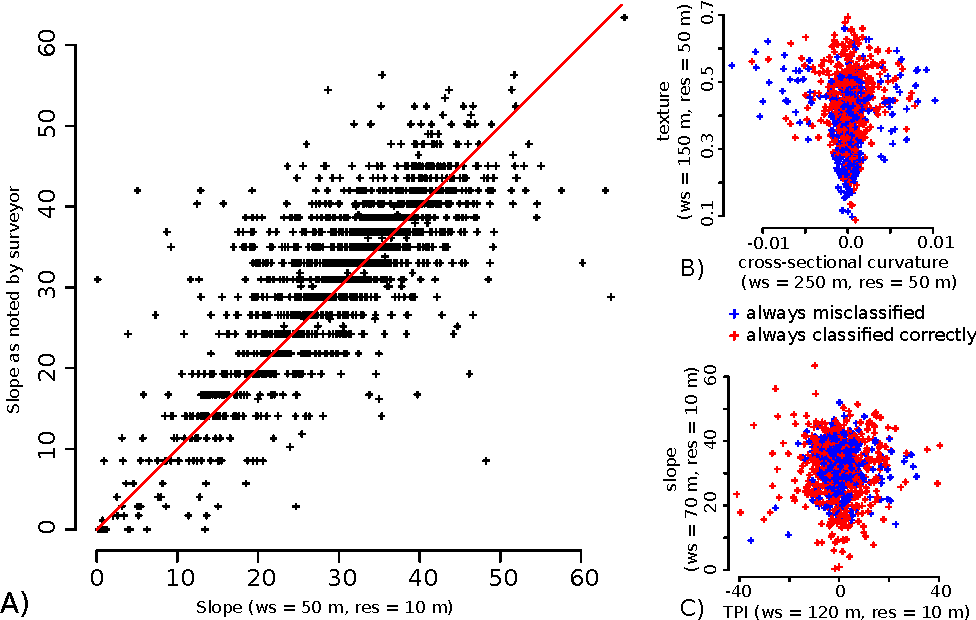
\includegraphics[width=\textwidth]{slope.pdf}
\caption{A) comparison of slope values of the soil pit site descriptions and the  values derived from the 10 m resolution DTM. The red line indicates were slope values should be if equal. B) and C) show scatter plots of the two terrain parameters that best differentiate the data points that were always classified correctly from those always misclassified, for macro and meso scale, respectively}
\label{fig:slope}
\end{figure}
 Figure \ref{fig:slope} gives an overview of the most influential terrain parameters identified for macro and meso scale, as well as a comparison of the slope gradient noted by the surveyor and that derived from the DTM. 

\begin{figure}
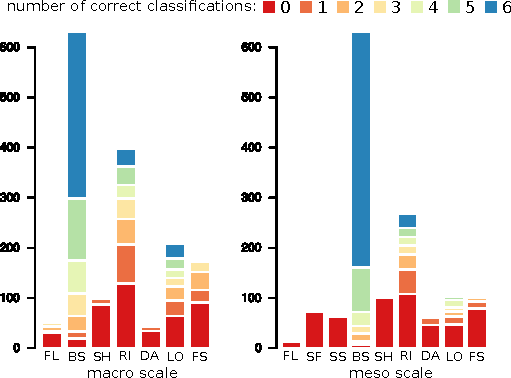
\includegraphics[width=\textwidth]{nr_correct_barplotperposition_EDITED_onlyGL1.pdf}
\caption{At each scale and generalisation level, a barplot shows the distribution of the number of times a specific data point was classified correctly using the six different methods.}
\label{fig:hist_correct_per_tp}
\end{figure}


\section{Discussion}
\subsection{Overall assessment of results}
All in all, the described methodology searches for parameter settings that best distinguish the topographic positions, leading to a trade-off between 1) landform maps with a large number of diverse classes where a dominant topographic position appropriates all modelled landform classes and 2) landform maps with very few modelled landform classes which are able to largely encompass the dominant topographic position but fail to differentiate the DTM enough to consider the less dominant topographic positions.
This study shows that, in the Alpine context, especially with the main land use being forestry, the reconstruction of topographic positions described by surveyors using terrain derivatives and classification schemes based on these, is possible only to a certain degree. The various investigated classification algorithms performed similarily at the  macro scale with 7 classes and at meso scale with 9 classes, yielding overall accuracies of just around 50\%.

Vielleicht hier noch welche klassen allgemein ein problem waren?

 Considering the often mentioned importance of topography in the soil surveyors mental soil landscape model, it is surprising that the topographic positions cannot be better replicated using simple terrain parameters or existing landform classification algorithm. What is more, the rule set on which surveyors classify topographic position is based on morphometric characteristics \citep{Englisch1998}. This raises several questions with regard to the reason for the presented results. The main issues that require discussion are (a) the quality of ground data, which is the reliability of point data regarding their location, (b) the field classification scheme, influenced by subjectivity and interpretability of the topographic position description performed by the soil surveyor, and (c) the properties of the used sample. A further issue that necessitates exploring is the adequacy of the examined classification algorithms with regard to their application in an Alpine environment. 
\paragraph{Reliability of individual profile points} 
Figure \ref{fig:hist_correct_per_tp} shows that at macro scale and generalisation level 1, a substantial amount of points, consisting of almost a third of the data set, were misclassified in every single classification approach. On the contrary, approximately the same number of data points were classified correctly in all six classification approaches. This indicates that only a third of the dataset is prone to changes in class due to the different approaches. So in summary, a third of the data points could not be correctly included into a single classification attempt. Possible reasons are explored in the following sections. Wrong coordinates due to limitations of global positioning system (GPS) accuracy under tree cover could be an explanation, however the use of coarser, resampled DTMs should take into account a large part of the uncertainty of maximum 50 m as conveyed by discussions with surveyors, especially at macro scale. The consistent effect of grid cell size regarding the difference between topographic position at macro and meso scale reported farther below, indicates that, while indivual points may be incorrectly localised, there is no systematic error in the localisation of the profile sites. Otherwise the DTM resolution or chosen window size should show no correlation with the extents that are used in the survey manual to distinguish meso and macro scale. Consequently, other issues at the least contribute to the large number of points that cannot be classified correctly. Figure \ref{fig:slope} B) and C) show that those points always misclassified at macro scale are often characterized by high texture values, indicating rough or steep terrain. At meso scale, the consistently misclassified point surround the correctly classified points which center around a TPI of 0 and a slope of around 30$^{\circ}$, which well characterizes the backslope position. These scatterplots are indicative of the issues that arise in Alpine terrain and are discussed in the following sections.
\paragraph{Objectivity of topographic position description and classification}
\cite{Congalton1991} notes that a classification system should be mutually exclusive and exhaustive, however with topographic positions and landforms there are not clear and crisp boundaries. The differences and transitions between different positions are open to interpretation by the individual surveyor. A remarkable aspect of the surveyed topographic positions of the soil profile sites (figure \ref{fig:hist}) is the dominance the backslope class, which is present at macro scale and even more at meso scale. However, given the Alpine environment in which the survey was performed, this is not unjustifiable. The low overall classification rate can be partly attributed to the generally high rate of misclassifications of other positions as backslope due to the great range of the terrain parameters found at positions classified as such. \cite{Brevik2015} note the important influence landscape has on what the surveyor sees when describing a soil profile. Although this statement presumably refers to the undeniable influence of topography on soil formation, it can also be (mis)interpreted as describing the effect of the soil surveyors personal mental soil-landscape model on which soil or horizon characteristics are observed in situ. One hypothesis could be that this relationship goes in both directions, meaning that what the surveyor observes in the soil pit may also reflect on his perception of topographic position due to his expectation of where such soils can be found. For instance, many soils in an Alpine environment are formed from multi-layered deposits \citep{Baruck2015,Geitner2011a}, consequently the backslope position with its dynamic equilibrium of erosion and sedimentation would seem an appropriate topographic position for such soils. A further plausible situation leading to an abundance of backslopes in the profile site data set, is that the backslope position is the ``go-to'' class that is attributed to a profile site which does not convincingly fit the descriptions of any of the other topographic positions available in the survey manual. The possibility of any of these two situations to arise is further increased by limited visibility of the surrounding landscape as a consequence to the profile sites' location in partly densely vegetated forests. It must further be noted that the data point description stems from various surveyors, each with his own mental landscape model. \cite{Matsuura2012} compared the results of their breakline detection-based slope segmentation model with maps prepared by manual interpretation of slope contours. They attribute the reported deviations among the manual delineations to differences in the human interpreters definitions of slope segments, especially regarding lower, mid and upper slopes. If these differences are present even in situations were the human interpreter has a good overview of the larger topographic situation, as is the case when using slope contours, it is likely that these differences are similar or even greater in field survey, with possibly impaired visibility as mentioned above. Two classes used in our study where we particularily estimate the subjectivity and non-exclusivity of topographic positions to be  an issue are slope flattening and slope steepening, which are only included at meso scale. However, none of the six approaches exemplified in this study managed to replicate these topographic positions, presumably due to the very fuzzy definition of these positions, especially when competing with the backslope position and its wide terrain parameter ranges.
\paragraph{The point sample regarding topographic position}
Although the authors were not part of one of the various survey teams and thus not involved in the sampling scheme, this issue must also be addressed. Parts of the data can be seen as part of a stratified sampling scheme, however not with regard to topographic position but forest types. It cannot be termed random stratified sampling, as the profile points were selected on practical criteria, especially the proximity to forestry service roads. Due to the focus on forest types, certain topographic positions, for instance valley floor and debris fans or cones, were undersampled, as these positions are dominated by agriculture and not forests. An additional field campaign based on random stratified sampling and including land uses other than forestry, would help to better capture the topographic variability of these positions and strengthen their position in the model. As discussed above,the backslope position dominates the sample and leads to an unbalanced data set, however \cite{Congalton1991} advises increased sample sizes for classes with high variability.


\subsection{Differences in meso and macro scale}
While the overall performance of the classification of topographic position was rather poor, the applied methodology does a considerably better job at highlighting the differences between topographic positions at macro and meso scale with regard to DTM resolution.
Regarding the algorithms were, as is the case with Dikau's curvature classification and Schmidt's fuzzy elements, grid cell size controls the scale of the are that is considered for calculating the relevant terrain parameters, the classifications that best fit the topographic positions at macro scale were also chosen from a coarser DTM than those for meso scale. While the macro scale classification using Dikau's curvature classification is based on the 100 m grid cell size DTM, Schmidt's fuzzy elements preferred an even coarser resolution of 150 m. Considering that the calculation of the the local terrain attributes regards a neighborhood of 3 grid cells, the involved area has an extent of 300 m and 450 m for Dikau's and Schmidt's classifications, respectively. According to the survey manual \citep{Englisch1998}, an extent of 100 - 500 m should be regarded for macro scale topographic positions, which is well in line with the 300 and 450 m. The manual describes meso scale topographic positions as having an extent fo 50 to 100 m, which agrees with the 50 m grid DTM chosen by Dikau's and Schmidt's algorithms, although the considered 3 grid cells amount to a slightly larger extent.
The other set of classification approaches investigated have a different option to incorporate scale into their computation. While Wood's classification can change the window size for which the local terrain parameters are calculated, the TPI-based landform uses two search radii for which the regional parameter is calculated whereas the geomorphon-based approach has one search radius for which the line-of-sight calculations are performed. The three approaches could furthermore choose betweeen the 10 and the 50 m DTM. For macro scale topographic positions, Wood's and the geomorphon approach went with the 50 m DTM while the TPI-based approach used the 10 m grid cell size. The window size or outer search radius for Wood's, the TPI-based and the geomorphon-based approaches were 250, 250 and 400 m, respectively. As with the two other grid cell size - driven approaches, these values are well within the range of the surveyor manuals macro scale definition. For the DTM resolution used for meso scale positions, all three search window-driven approaches went with the 10 m DTM and outer search radii or window sizes of 110, 90, and 80 m, respectively. The change in chosen DTM resolution from macro to meso scale is present in all but one method, and the extent of the meso scale topographic positions, as defined for the surveyors, is well reproduced in the search radii and grid cell sizes.
Considering the overall classification result at generalisation level1, there is no significant difference between meso and macro scale, although it must be noted that at meso scale two additional classes, slope steepening and slope flattening, which were however never replicated in the resulting maps, as mentioned previously.


\subsection{Performance of the different algorithm groups}  
The overall accuracies of best parameter setting of each classification approach do not differ as much as expected, presumably because all are calibrated toward the same data set. Due to the overwhelming variability of the backslope class as assigned by the surveyors, all approaches had difficulties with distinguishing smaller classes, especially seperating shoulder and footslope from backslope positions, but this problem seems data- and semantics-related. However, some deficiencies of the various classification algorithms were detected.
The approach with the best performance, the classifier based on a combination of single terrain parameters, also gives the most insight into what features apprear to have the greatest influence on the surveyors perception of his position in the landscape. 
All in all, at meso scale only 3 positions were usually mapped!! and also for macro sh and fs hardly ever.

\subsection{The effect of the Alpine environment on the chosen parameter values} 
Most of the evaluated automatic classification algorithm include a slope threshold or fuzzy membership function that determines whether a grid cell is flat or sloped. Similarly, a large number include a curvature threshold or fuzzy membership function responsible for the classification as planar. The slope values chosen for the various classification methods in the methodology are consistently much higher than those found in literature or the default values of the software used. While most of the studies performing landform classification (for instance \cite{Barka2011}, \cite{Bocco2001}, \cite{Ehsani2008}, \cite{Jasiewicz2013}, \cite{MacMillan2000a}) apply thresholds of 2 or 3$^{\circ}$, or fuzzy membership functions approximately centering on these values, the presented methodology chose values between 8 and 10$^{\circ}$ for the geomorphon-based classification and between 11 and 15$^{\circ}$ for Wood's features. The same trend was noted regarding the choice of curvature, where much higher higher values were allowed for planar grid cells than expected from published studies. Only \cite{Schmidt2004} apply fuzzy membership functions for slope and curvature that show overlap with the values chosen in this study. However, most of the studies applying one or more of the discussed landforms do not concentrate on high relief areas such as South Tyrol. The authors of this study attribute the choice of high slope and curvature values to the steep relief in the study area and the under-representation of valley floor and similarly flat topographic positions in the data set. Higher slope  thresholds allow for better differentation of sloping areas, which is where the majority of the profile sites are situated. Some studies that include areas with high relief \citep{Bocco2001,Herbst2012} deal with this issue by adjusting their flatness threshold for plateaus. This underlines the necessity of adapting slope and curvature thresholds or membership functions to the topography in the area of interest, especially in an Alpine environment. Considering the discussion on the objectivity of topographic position descriptions above, what is considered to be sloping in hummocky terrain could be considered flat regarding morphodynamics in an Alpine context, especially in the perception of a soil surveyor while performing field work. A comparison of the slope gradient as described during field survey with the slope gradient derived from a DTM at various window sizes showed the best fit with a window size of 50 m based on the 10 m grid. A scatterplot of the two slope gradients values shows that, while an overall agreeing trend can be observed, there is often a substantial difference between the slope gradient perceived by the surveyor and the one derived digitally. Whereas points with an exceedingly large difference in slope indicate issues regarding the uncertainty of the profile site location, the scatterplot does suggest larger deviations in steeper terrain, further illustrating the influence the high relief environment has on how the human surveyor perceives and evaluates his position in the landscape. 

\subsection{Support vector machine classification and parameter selection}
While there exist simpler statistics to compare two maps, for instance those based on the $\chi^2$ coefficient, the machine learning approach was chosen so that we could investigate the most influential terrain parameters for replicating the surveyor's perception of topographic position by constructing a model using  SVM classification. To reduce the number of methods and for the sake of comparability, this approach was also applied for selecting the best fitting parameter settings for each of the applied automated classifications. Next to advancing the understanding of the surveyors perception of landscape with regard to his mental soil landscape model, the creation of a map of modeled topographic position to aid soil surveyors in the field was an additional goal, especially in light of the results presented in this study. With regard to different machine learning approaches, for instance random forest classification \citep{Breiman2001}, SVM classification was chosen for its ability to create smooth prediction surfaces, for, as noted by \cite{Steger2016}, these improve the readability and hence utility of maps for practical purposes, for instance soil survey.

As most landform classification algorithms in themselves already involve the classification and generalisation of various terrain parameters, classification power was rarely increased by the combination of result maps of the same classification scheme applying different parameter settings or scale, for instance combining two geomorphon-based landform maps computed with different search radii. The assumption is that this is because the aim of the procedure is to recreate topographic a position at a very specific scale, which is meso or macro scale as defined in the survey manual. When building a model through forward selection of single terrain parameters however, the classification results did improve. Generally, this improvement abated after a feature set of  three to four terrain parameters had been selected. While the addition of several parameters may have slightly increased the classification accuracy, it must be kept in mind that the aim of the procedure is to find some basic knowledge regarding the perception of the landscape by the surveyor and not to overfit our model to the dataset by using many features.
\section{Conclusion}
\section*{Acknowledgements} This research was performed within the project ``Terrain Classification of ALS Data to support Digital Soil Mapping'', funded by the Autonomous Province Bolzano -- South Tyrol (15/40.3).
\section*{References}
\bibliography{p1.bib}

\end{document}